\subsection{การทดลองการเดิน}
การทดลองการเดินนั้นได้ทดลองด้วยการปรับค่าข้อต่อให้เหมาะสมแก่การเดิน เพื่อทดสอบโครงสร้างที่ได้ออกแบบ
มาว่าสามารถรองรับการเดินของหุ่นยนต์ได้จริงหรือไม่ โดยค่าที่ใช้ในการปรับนั้นจะเป็นค่ามุมของมอเตอร์ส่วนต่างๆของส่วนขาทั้ง 2 ข้าง
โดยจะตั้งชื่อมอเตอร์ให้เป็นหมายเลขทั้ง 12 หมายเลข ซึ่งหมายเลขของขาด้านขวาจะเป็นหมายเลข 1-6 และหมายเลขของขาด้านซ้าย คือ 6-12
ในการปรับค่านั้นจะทดลองปรับค่าด้วยการมองท่าทางการขยับของหุ่นยนต์แล้วค่อยๆปรับค่าให้เหมาะสมเพื่อให้หุ่นยนต์ทรงตัวได้ โดยค่าที่ใช้ในการสั่ง
\begin{figure}[!ht]
    \centering
    \begin{subfigure}[b]{0.4\linewidth}
      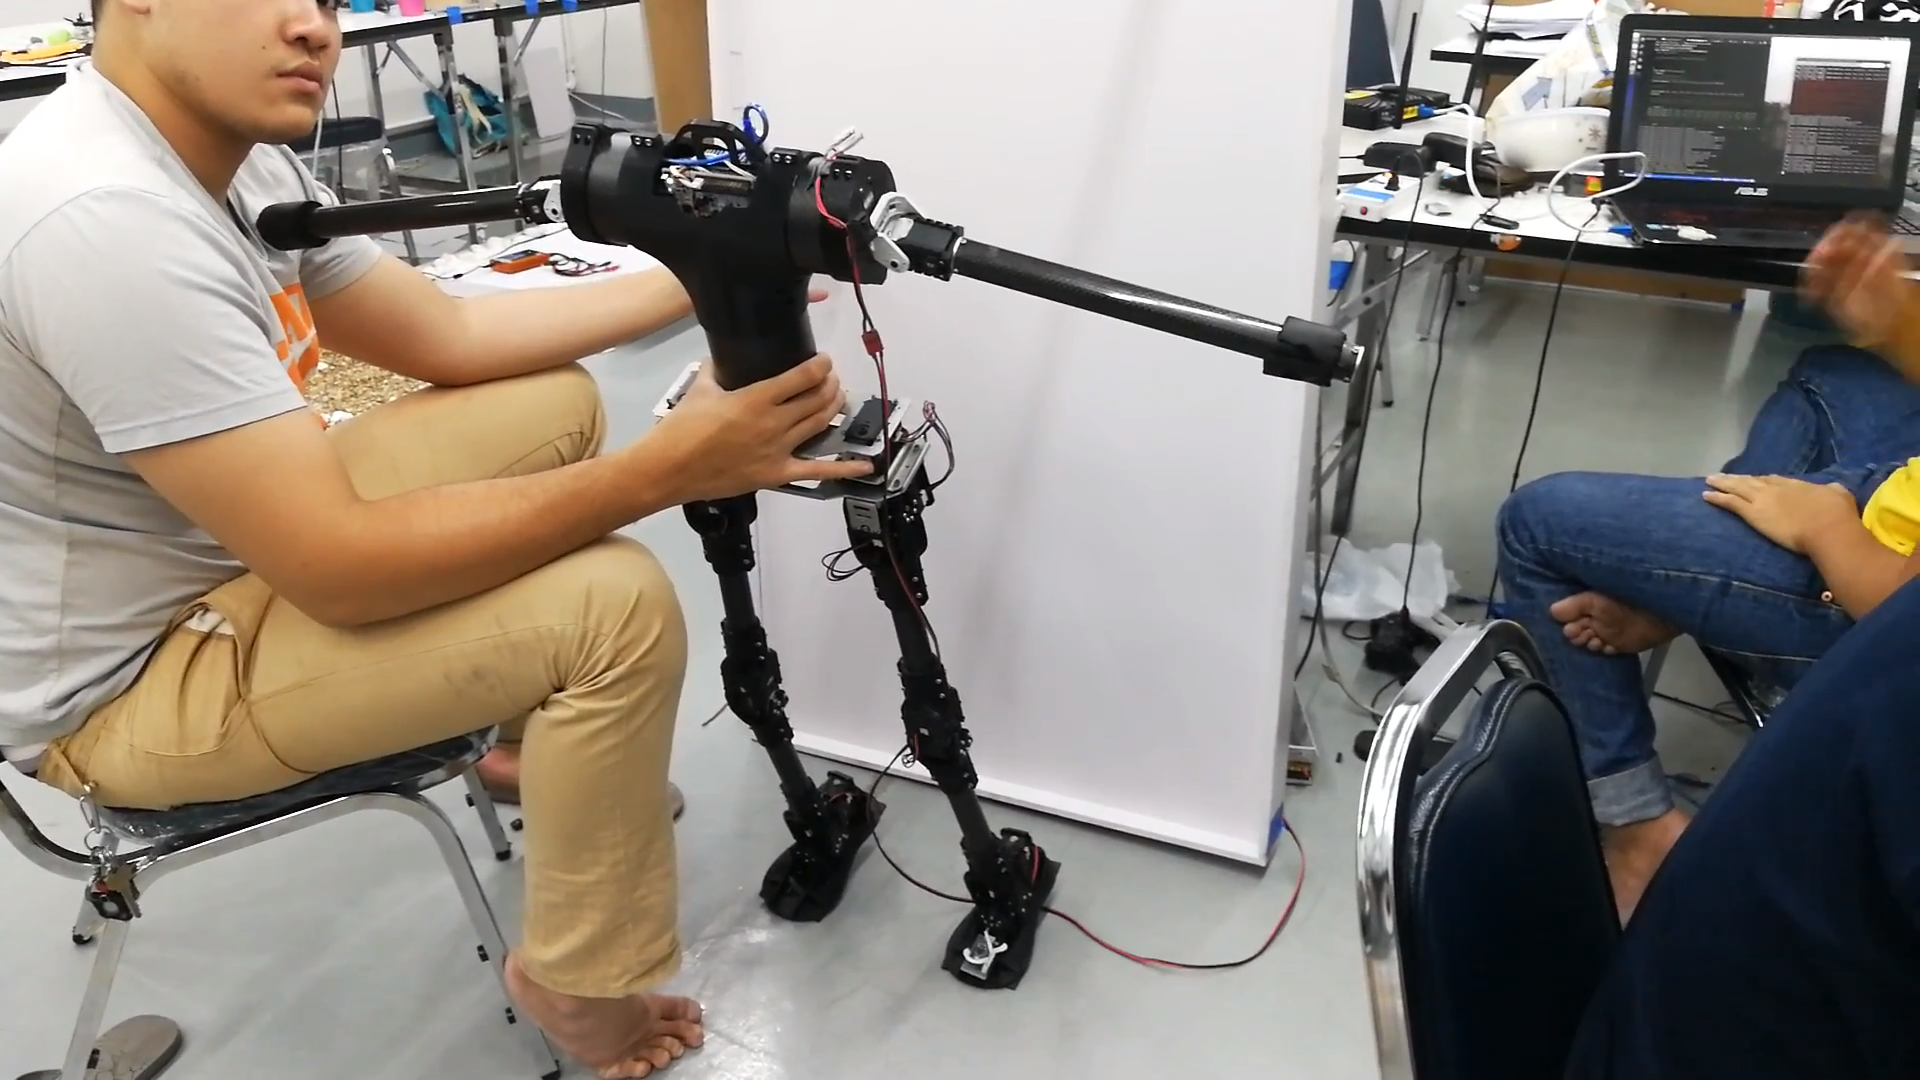
\includegraphics[width=\linewidth]{chapter4/images/fall1.png}
      \caption{รูปการล้มครั้งที่ 1}
    \end{subfigure}
    \begin{subfigure}[b]{0.4\linewidth}
      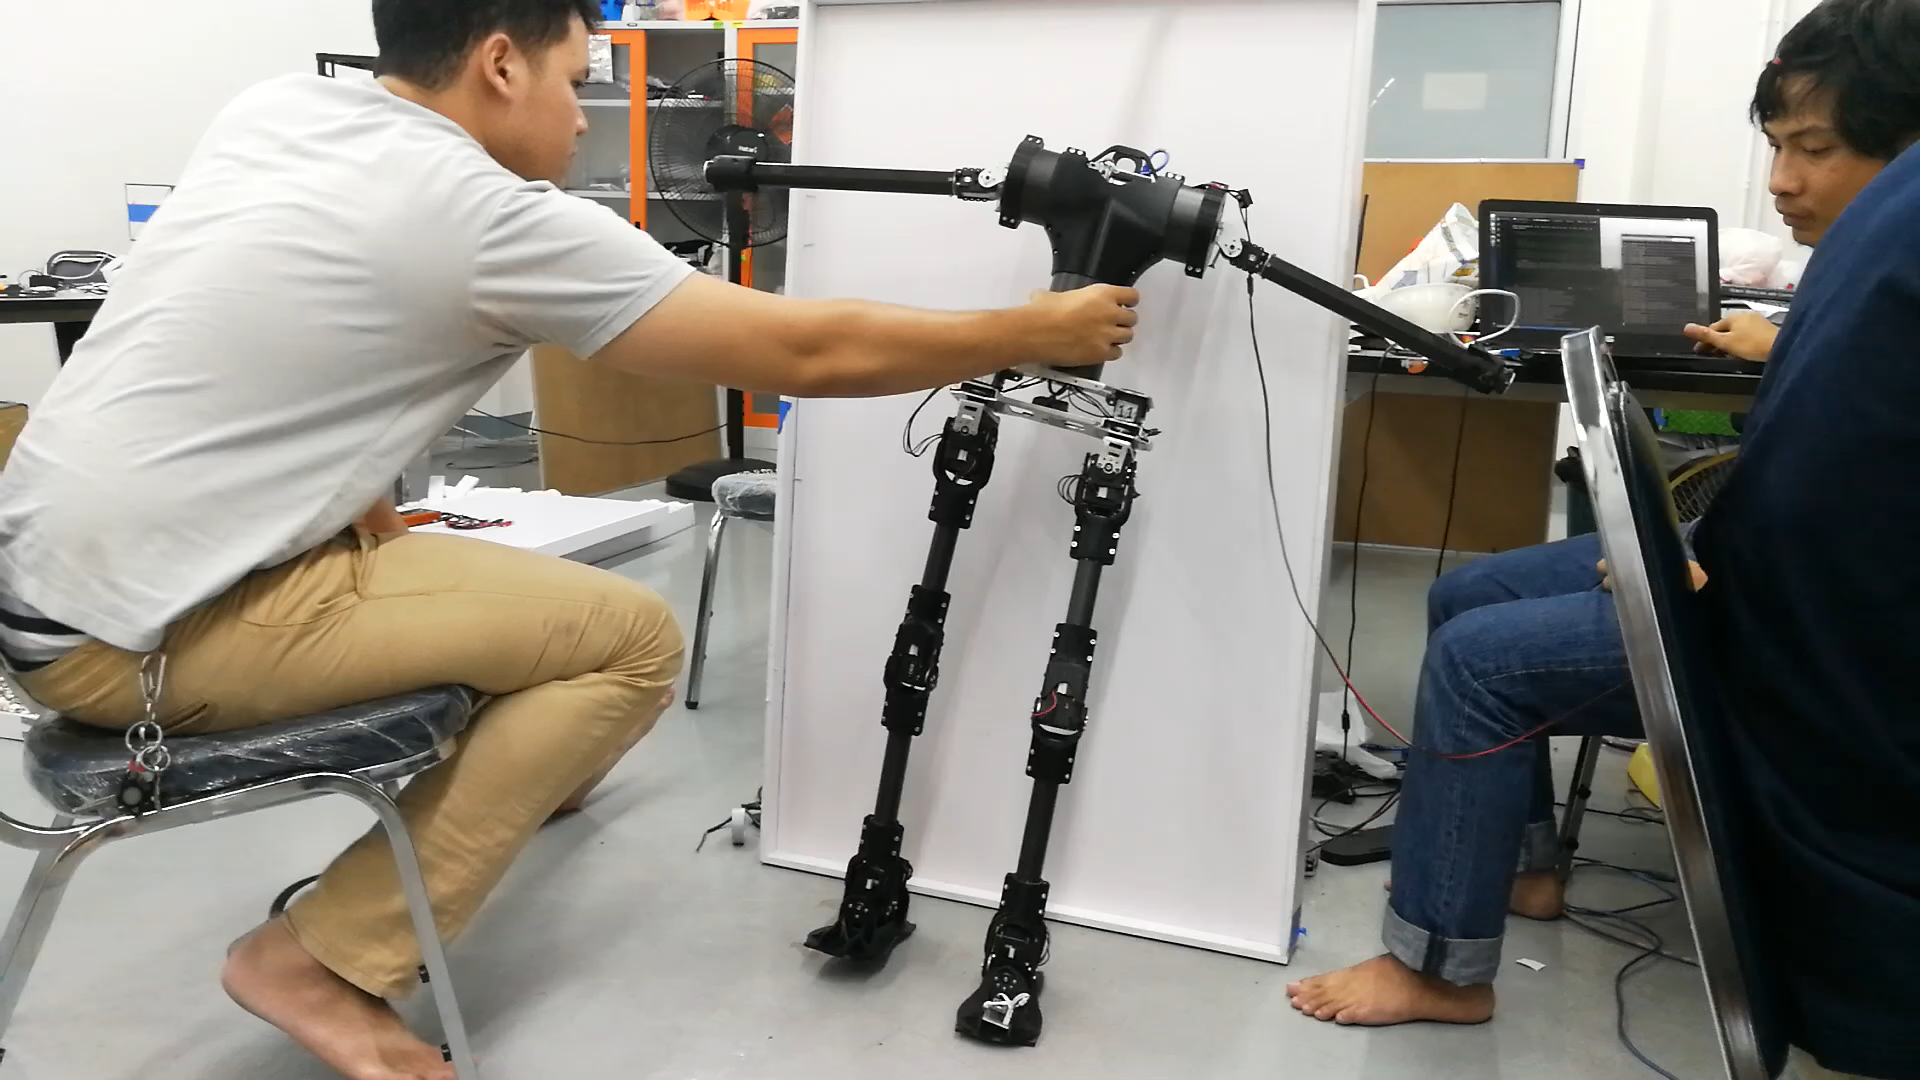
\includegraphics[width=\linewidth]{chapter4/images/fall2.png}
      \caption{รูปการล้มครั้งที่ 2}
    \end{subfigure}
    \begin{subfigure}[b]{0.4\linewidth}
      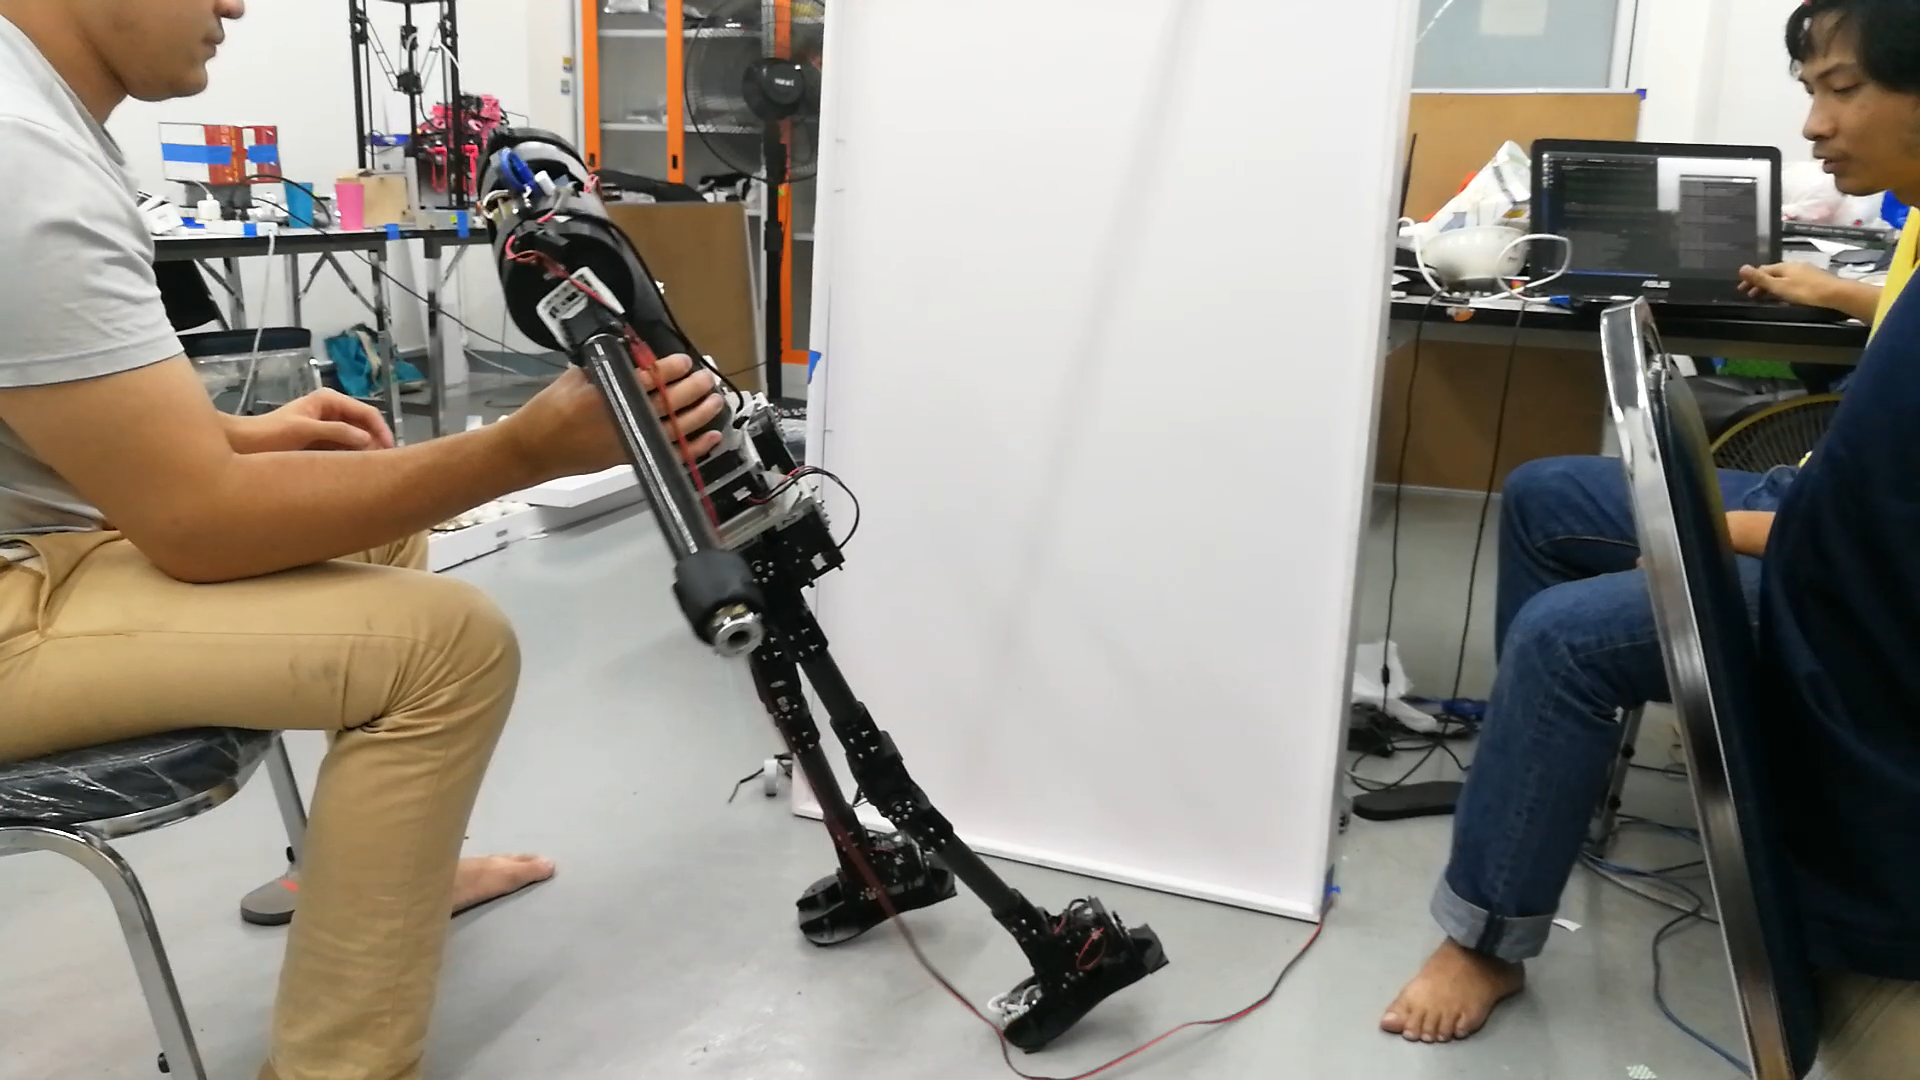
\includegraphics[width=\linewidth]{chapter4/images/fall3.png}
      \caption{รูปการล้มครั้งที่ 3}
    \end{subfigure}
    \begin{subfigure}[b]{0.4\linewidth}
      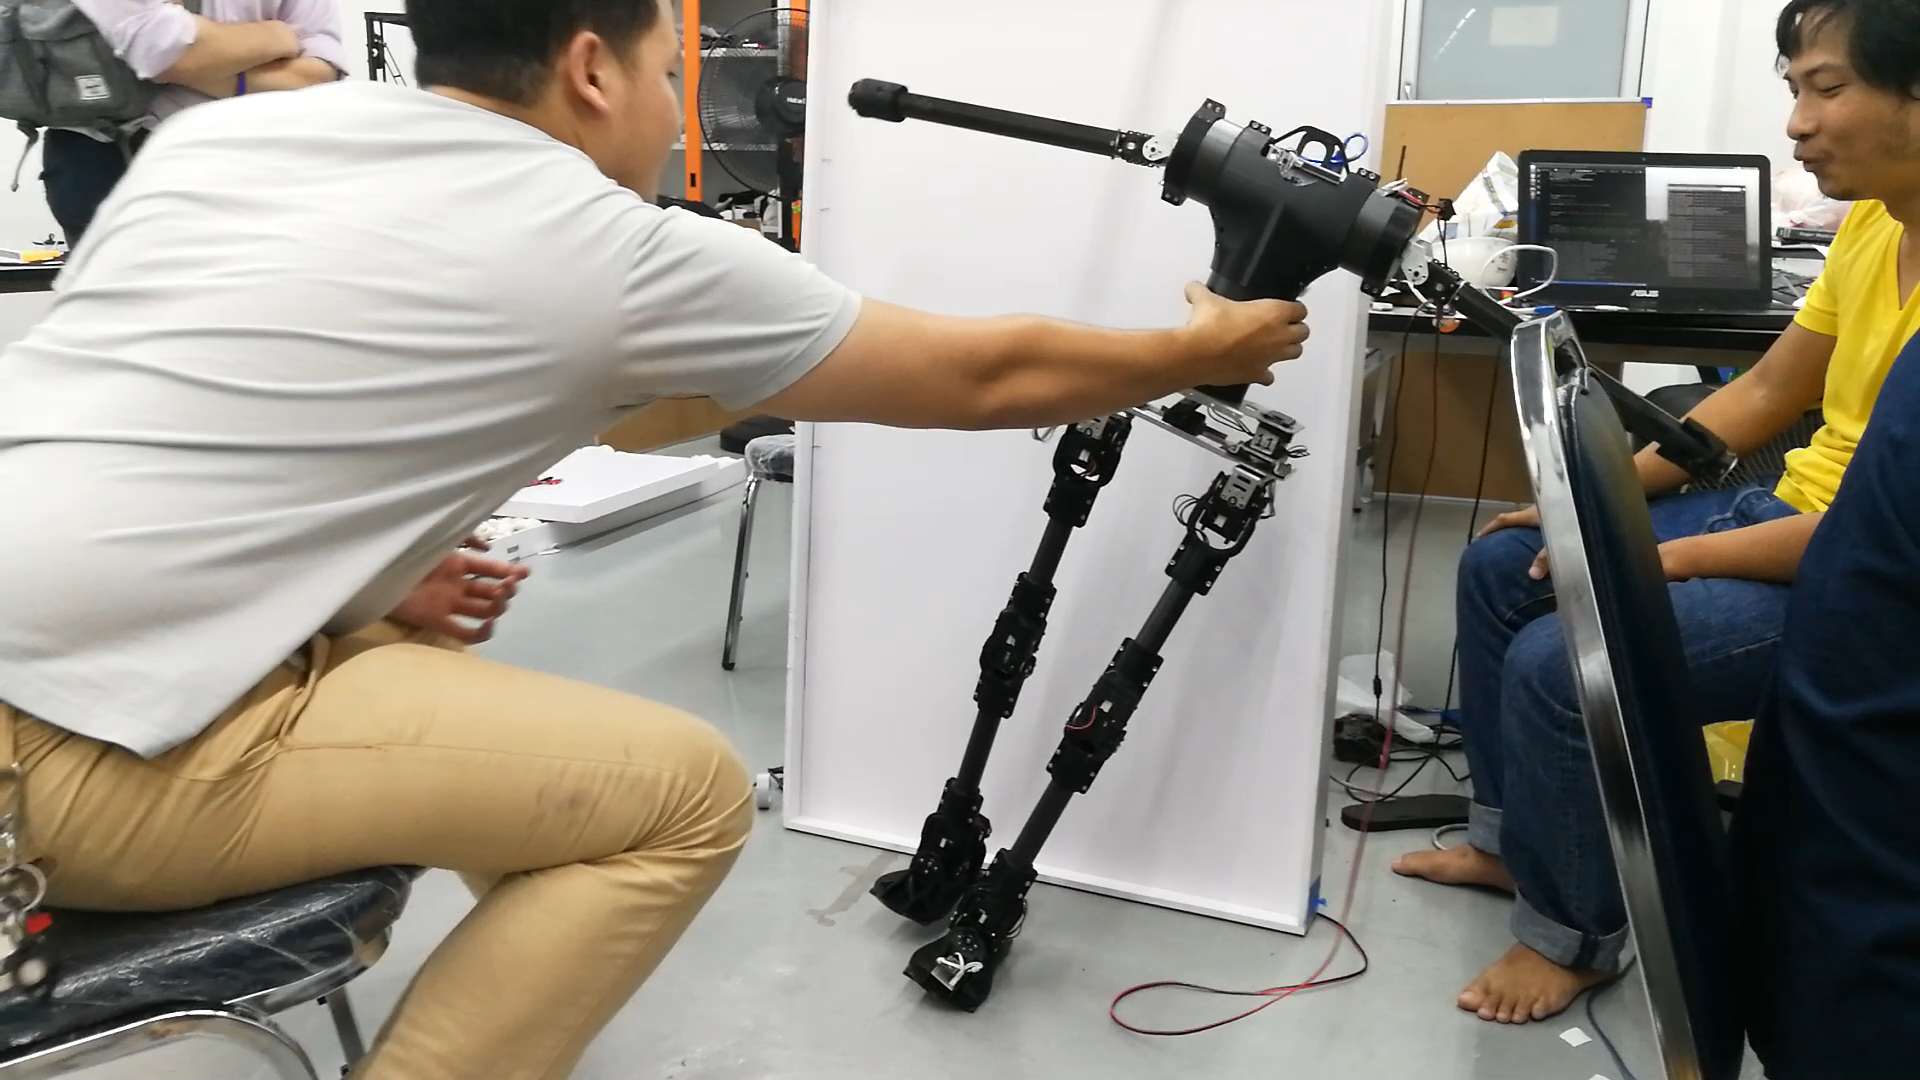
\includegraphics[width=\linewidth]{chapter4/images/fall4.png}
      \caption{รูปการล้มครั้งที่ 4}
    \end{subfigure}
    \begin{subfigure}[b]{0.4\linewidth}
      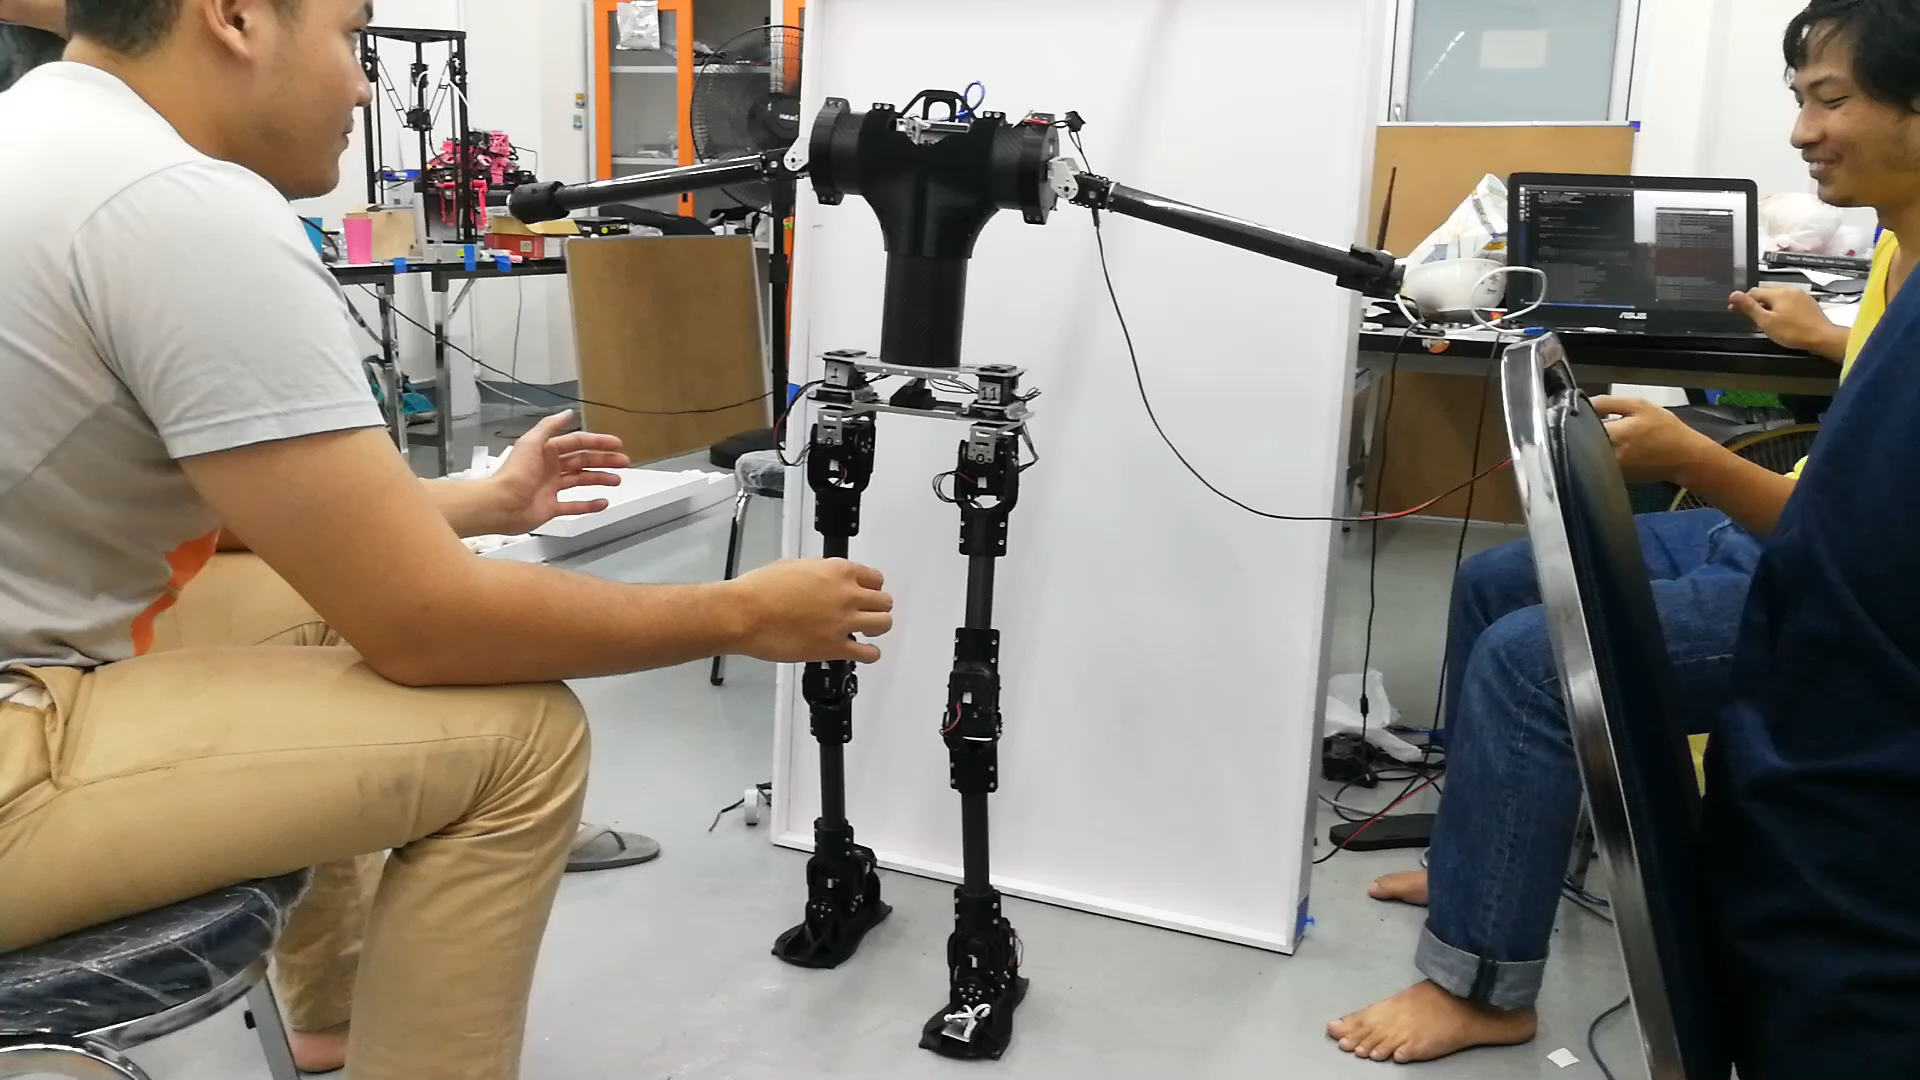
\includegraphics[width=\linewidth]{chapter4/images/achive1.png}
      \caption{รูปการก้าวสำเร็จ}
    \end{subfigure}
    \caption{รูปการทดลองการเดินของหุ่นยนต์ UTHAI}
    \label{fig:test_result}
  \end{figure}

% มอเตอร์ให้ขยับจะเป็นค่าของมุม(เรเดียล) และความเร็วในการถึงมุมที่กำหนด(วินาที) โดยมีค่าที่ทดลองดังนี้
% \begin{table}[!ht]
% 	\centering
% 	\begin{tabular}{| c | l | l | l | l | l |}
% 		\hline
% 		มอเตอร์ตัวที่ & มุม/เร็ว 1 & มุม/เร็ว 2 & มุม/เร็ว 3 & มุม/เร็ว 4 & มุม/เร็ว 5 \\
%         \hline
%         1 & & & & & \\
%         2 & & & & & \\
%         3 & & & & & \\
%         4 & & & & & \\
%         5 & & & & & \\
%         6 & & & & & \\
%         7 & & & & & \\
%         8 & & & & & \\
%         9 & & & & & \\
%         10 & & & & & \\
%         11 & & & & & \\
%         12 & & & & & \\
%         ผลการเดิน & & & & & \\
% 	    \hline
% 	\end{tabular}
% 	\caption{ตารางทดลองค่ามุมของมอเตอร์สำหรับการเดิน ก้าวแรก}
% 	\label{tab:First_step}
% \end{table}  


\clearpage
\subsection{ปัญหาที่พบ}
\subsubsection{อุณหภูมิ}
เมื่อมีการใช้งานเป็นเวลานานจะส่งผลให้มอเตอร์ส่วนสะโพกและข้อเท้ามีความร้อนสูงถึง 50 องศาเซลเซียส 
เนื่องจากมีการสั่งงานให้มอเตอร์อยู่ในตำแหน่งที่กำหนด ซึ่งเมื่อมีแรงบิดข้างนอกมาเกี่ยวข้อง จะทำให้มอเตอร์นั้น
พยายามรักษามุมของตนเองไว้ ส่งผลให้เกิดความร้อนเกิดขึ้นและ ส่งผลให้มอเตอร์อ่อนแรงลงเนื่องจากความร้อนที่เกิดขึ้น 
ในการแก้ไขปัญหานี้สามารถเพิ่มเติมส่วนของการระบายอากาศซึ่งจะส่งผลให้ตัวของหุ่นยนต์นั้นมีน้ำหนักมากขึ้น หรือ หยุดการทดลอง
ไว้สักระยะเพื่อให้มีการระบายอากาศให้อยู่ในอุณหภูมิปกติ
\subsubsection{โครงสร้าง}
เนื่องจากการยึดท่อคาร์บอนไฟเบอร์นั้นได้ทำการยึดด้วยการบีบอัดเพื่อให้เกิดแรงเสียดทางสูงแต่ว่าเมื่อมีการ สั่งงานที่มีการกระชากกล่าวคือ
มีการเคลื่อนที่ของมุมมอเตอร์ที่มีความแร็วสูง จะส่งผลให้เกิดแรงบิดตามแนวแกนซึ่งเกินแรงเสียดทานที่การยึดติดจะรับไหว จึงเกิดการบิด ของข้อต่อ
เกิดขึ้น ส่งผลให้ ส่วนของเท้ามีการบิดไปจากท่าปกติ ซึ่งสามารถแก้ไขได้โดยเพิ่มแรงยึดด้วยการเสริมแผ่นยางบางๆบริเวณหน้าสัมผัสที่ติดกับท่อคาร์บอนไฟเบอร์
เพื่อเพิ่มแรงยึดไปอีกขั้นหนึ่ง 


